% =============================================================
% Project 1 Presentation (ROS 2 + Gazebo + SLAM + Nav2)
% Format aligned with OS_slide
% =============================================================
\documentclass[aspectratio=169]{beamer}

% --- Theme Selection ---
\usetheme{Madrid}
\usecolortheme{dolphin}

% --- Packages ---
\usepackage{graphicx}
\usepackage{booktabs}
\usepackage{tikz}
\usetikzlibrary{shapes, arrows, positioning, fit, calc, decorations.pathmorphing, shadows}
\usepackage{amsmath}

% --- Title Information ---
\title[Project 1: ROS 2 SLAM \& Nav2]{Project 1 Progress Report\\ROS 2 Jazzy + Gazebo + SLAM + Nav2}
\subtitle{Setup, Mapping, Navigation, and Extensions}
\author[Team/Student]{Kieu Son Tung}
\institute[HUST]{Hanoi University of Science and Technology (HUST)}
\date{\today}

\begin{document}

% Slide 1: Title
\begin{frame}
    \titlepage
\end{frame}

% Slide 2: Table of Contents
\begin{frame}{Outline}
    \tableofcontents
\end{frame}

% =============================================================
% Section: Environment Setup
% =============================================================
\section{Environment Setup}
\begin{frame}{1. System Environment}
    \begin{columns}[T]
        \column{0.62\textwidth}
        \textbf{Platform}
        \begin{itemize}
            \item Windows 11 + WSL2 (Ubuntu 24.04)
            \item ROS 2 Jazzy Jalisco
            \item Gazebo Harmonic (simulation)
            \item TurtleBot3 (Burger)
        \end{itemize}

        \vspace{0.3cm}
        \textbf{Goal:} Build a reproducible robotics workflow for SLAM and navigation experiments.

        \column{0.38\textwidth}
        \centering
        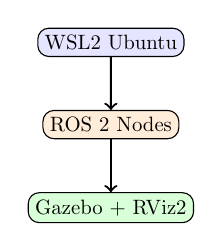
\begin{tikzpicture}[node distance=0.9cm, auto, scale=0.75, transform shape]
            \node[draw, rounded corners, fill=blue!10] (wsl) {WSL2 Ubuntu};
            \node[draw, rounded corners, fill=orange!15, below=of wsl] (ros) {ROS 2 Nodes};
            \node[draw, rounded corners, fill=green!15, below=of ros] (sim) {Gazebo + RViz2};
            \draw[->, thick] (wsl) -- (ros);
            \draw[->, thick] (ros) -- (sim);
        \end{tikzpicture}
        \vspace{0.2cm}
        \begin{block}{Key Output}
            Working simulation + tooling for later research.
        \end{block}
    \end{columns}
\end{frame}

% =============================================================
% Section: Simulation and Teleop
% =============================================================
\section{Simulation and Teleoperation}
\begin{frame}{2. Gazebo Simulation}
    \begin{columns}[T]
        \column{0.55\textwidth}
        \textbf{What we ran}
        \begin{itemize}
            \item TurtleBot3 world in Gazebo
            \item Teleop keyboard to drive the robot
            \item Sensor topics available (e.g., \texttt{/scan})
        \end{itemize}

        \vspace{0.3cm}
        \begin{block}{Result}
            Stable simulation environment ready for mapping and navigation.
        \end{block}

        \column{0.45\textwidth}
        \centering
        \includegraphics[width=\linewidth]{gazebo.png}
        \vspace{0.1cm}
        \footnotesize{Gazebo Harmonic simulation with TurtleBot3.}
    \end{columns}
\end{frame}

\begin{frame}{3. RViz2 Visualization}
    \begin{columns}[T]
        \column{0.55\textwidth}
        \textbf{RViz configuration}
        \begin{itemize}
            \item Fixed Frame: \texttt{odom} (teleop testing) / \texttt{map} (SLAM)
            \item Add \texttt{/scan} (LaserScan)
            \item Add RobotModel / TF for debugging
        \end{itemize}

        \vspace{0.3cm}
        \begin{block}{Why it matters}
            Quick feedback loop for sensor timing and frame consistency.
        \end{block}

        \column{0.45\textwidth}
        \centering
        \includegraphics[width=\linewidth]{rviz.png}
        \vspace{0.1cm}
        \footnotesize{Laser scan and robot model in RViz2.}
    \end{columns}
\end{frame}

% =============================================================
% Section: SLAM
% =============================================================
\section{SLAM Mapping}
\begin{frame}{4. SLAM Toolbox (Online Async)}
    \textbf{Mapping workflow}
    \begin{enumerate}
        \item Launch SLAM Toolbox (online async) and drive the robot to explore.
        \item SLAM performs scan matching and pose-graph updates.
        \item Publish occupancy grid map (\texttt{/map}) for later use.
    \end{enumerate}

    \vspace{0.4cm}
    \begin{columns}
        \column{0.52\textwidth}
        \begin{block}{Deliverable}
            A complete map that can be saved and reused for Nav2 navigation.
        \end{block}
        \column{0.48\textwidth}
        \centering
        \includegraphics[width=\linewidth]{slam_done.png}
        \footnotesize{Completed SLAM map.}
    \end{columns}
\end{frame}

% =============================================================
% Section: Nav2
% =============================================================
\section{Autonomous Navigation (Nav2)}
\begin{frame}{5. Nav2 Bringup on the Saved Map}
    \begin{columns}[T]
        \column{0.56\textwidth}
        \textbf{Nav2 stack}
        \begin{itemize}
            \item Global planner: Dijkstra/A* on costmap (e.g., NavFn)
            \item Local controller: DWB for reactive obstacle avoidance
            \item Behavior Trees for task orchestration
        \end{itemize}

        \vspace{0.25cm}
        \begin{block}{Operation in RViz2}
            Set 2D Pose Estimate, then send Nav2 Goal to navigate.
        \end{block}

        \column{0.44\textwidth}
        \centering
        \includegraphics[width=\linewidth]{nav_load.png}
        \footnotesize{Nav2 initialized with the map loaded.}
    \end{columns}
\end{frame}

\begin{frame}{6. Navigation Result}
    \centering
    \includegraphics[height=0.72\textheight,keepaspectratio]{nav_path.png}
    \vspace{0.1cm}
    \footnotesize{The robot follows the planned path while the local planner avoids obstacles in real time.}
\end{frame}

% =============================================================
% Section: Programmatic Control
% =============================================================
\section{Programmatic Control}
\begin{frame}{7. Waypoint Navigation via Python}
    \textbf{Motivation:} Replace manual RViz testing with a repeatable program interface.
    \vspace{0.2cm}

    \textbf{Approach:}
    \begin{itemize}
        \item Use \texttt{nav2\_simple\_commander} (\texttt{BasicNavigator})
        \item Send goals or follow a list of waypoints
        \item Monitor completion to build automation scripts
    \end{itemize}

    \vspace{0.35cm}
    \begin{block}{Result}
        The robot can patrol through predefined positions without manual intervention.
    \end{block}
\end{frame}

% =============================================================
% Section: OS Resource Management (from extended work)
% =============================================================
\section{OS Resource Management (Extension)}
\begin{frame}{8. Why Resource Contention Matters}
    \begin{columns}[T]
        \column{0.55\textwidth}
        \textbf{Problem}
        \begin{itemize}
            \item ROS 2 nodes are OS processes competing for CPU time (CFS fairness).
            \item Under load, SLAM may process delayed scans $\rightarrow$ map drift.
        \end{itemize}
        \vspace{0.25cm}
        \begin{alertblock}{Impact}
            Once the map drifts, navigation quality degrades severely.
        \end{alertblock}

        \column{0.45\textwidth}
        \centering
        \includegraphics[width=\linewidth]{drift.png}
        \footnotesize{Example drift under contention.}
    \end{columns}
\end{frame}

\begin{frame}{9. Bandit vs. Q-Learning (High Level)}
    \begin{columns}[T]
        \column{0.49\textwidth}
        \centering
        \textbf{Bandit ($\epsilon$-greedy)}\\
        \vspace{0.15cm}
        \includegraphics[width=\linewidth]{bandit.png}
        \vspace{0.1cm}
        \footnotesize{Stateless: learns a single best action on average.}

        \column{0.49\textwidth}
        \centering
        \textbf{Q-Learning (State-Aware)}\\
        \vspace{0.15cm}
        \includegraphics[width=\linewidth]{Q.png}
        \vspace{0.1cm}
        \footnotesize{Stateful: reacts earlier when jitter rises.}
    \end{columns}
\end{frame}

% =============================================================
% Section: Dynamic Obstacles + Nav2 (new module)
% =============================================================
\section{Dynamic Obstacles (New Module)}
\begin{frame}{10. Dynamic Obstacles with Nav2}
    \begin{columns}[T]
        \column{0.58\textwidth}
        \textbf{Objective}
        \begin{itemize}
            \item Make the environment more realistic with moving obstacles.
            \item Test Nav2 re-planning behavior during execution.
        \end{itemize}
        \vspace{0.2cm}
        \textbf{Implementation}
        \begin{itemize}
            \item Spawn and move box entities in Gazebo.
            \item Periodic pose updates (\texttt{ros\_gz\_sim set\_entity\_pose}).
            \item Integrated bringup: Gazebo + Nav2 + RViz + obstacles.
        \end{itemize}

        \column{0.42\textwidth}
        \centering
        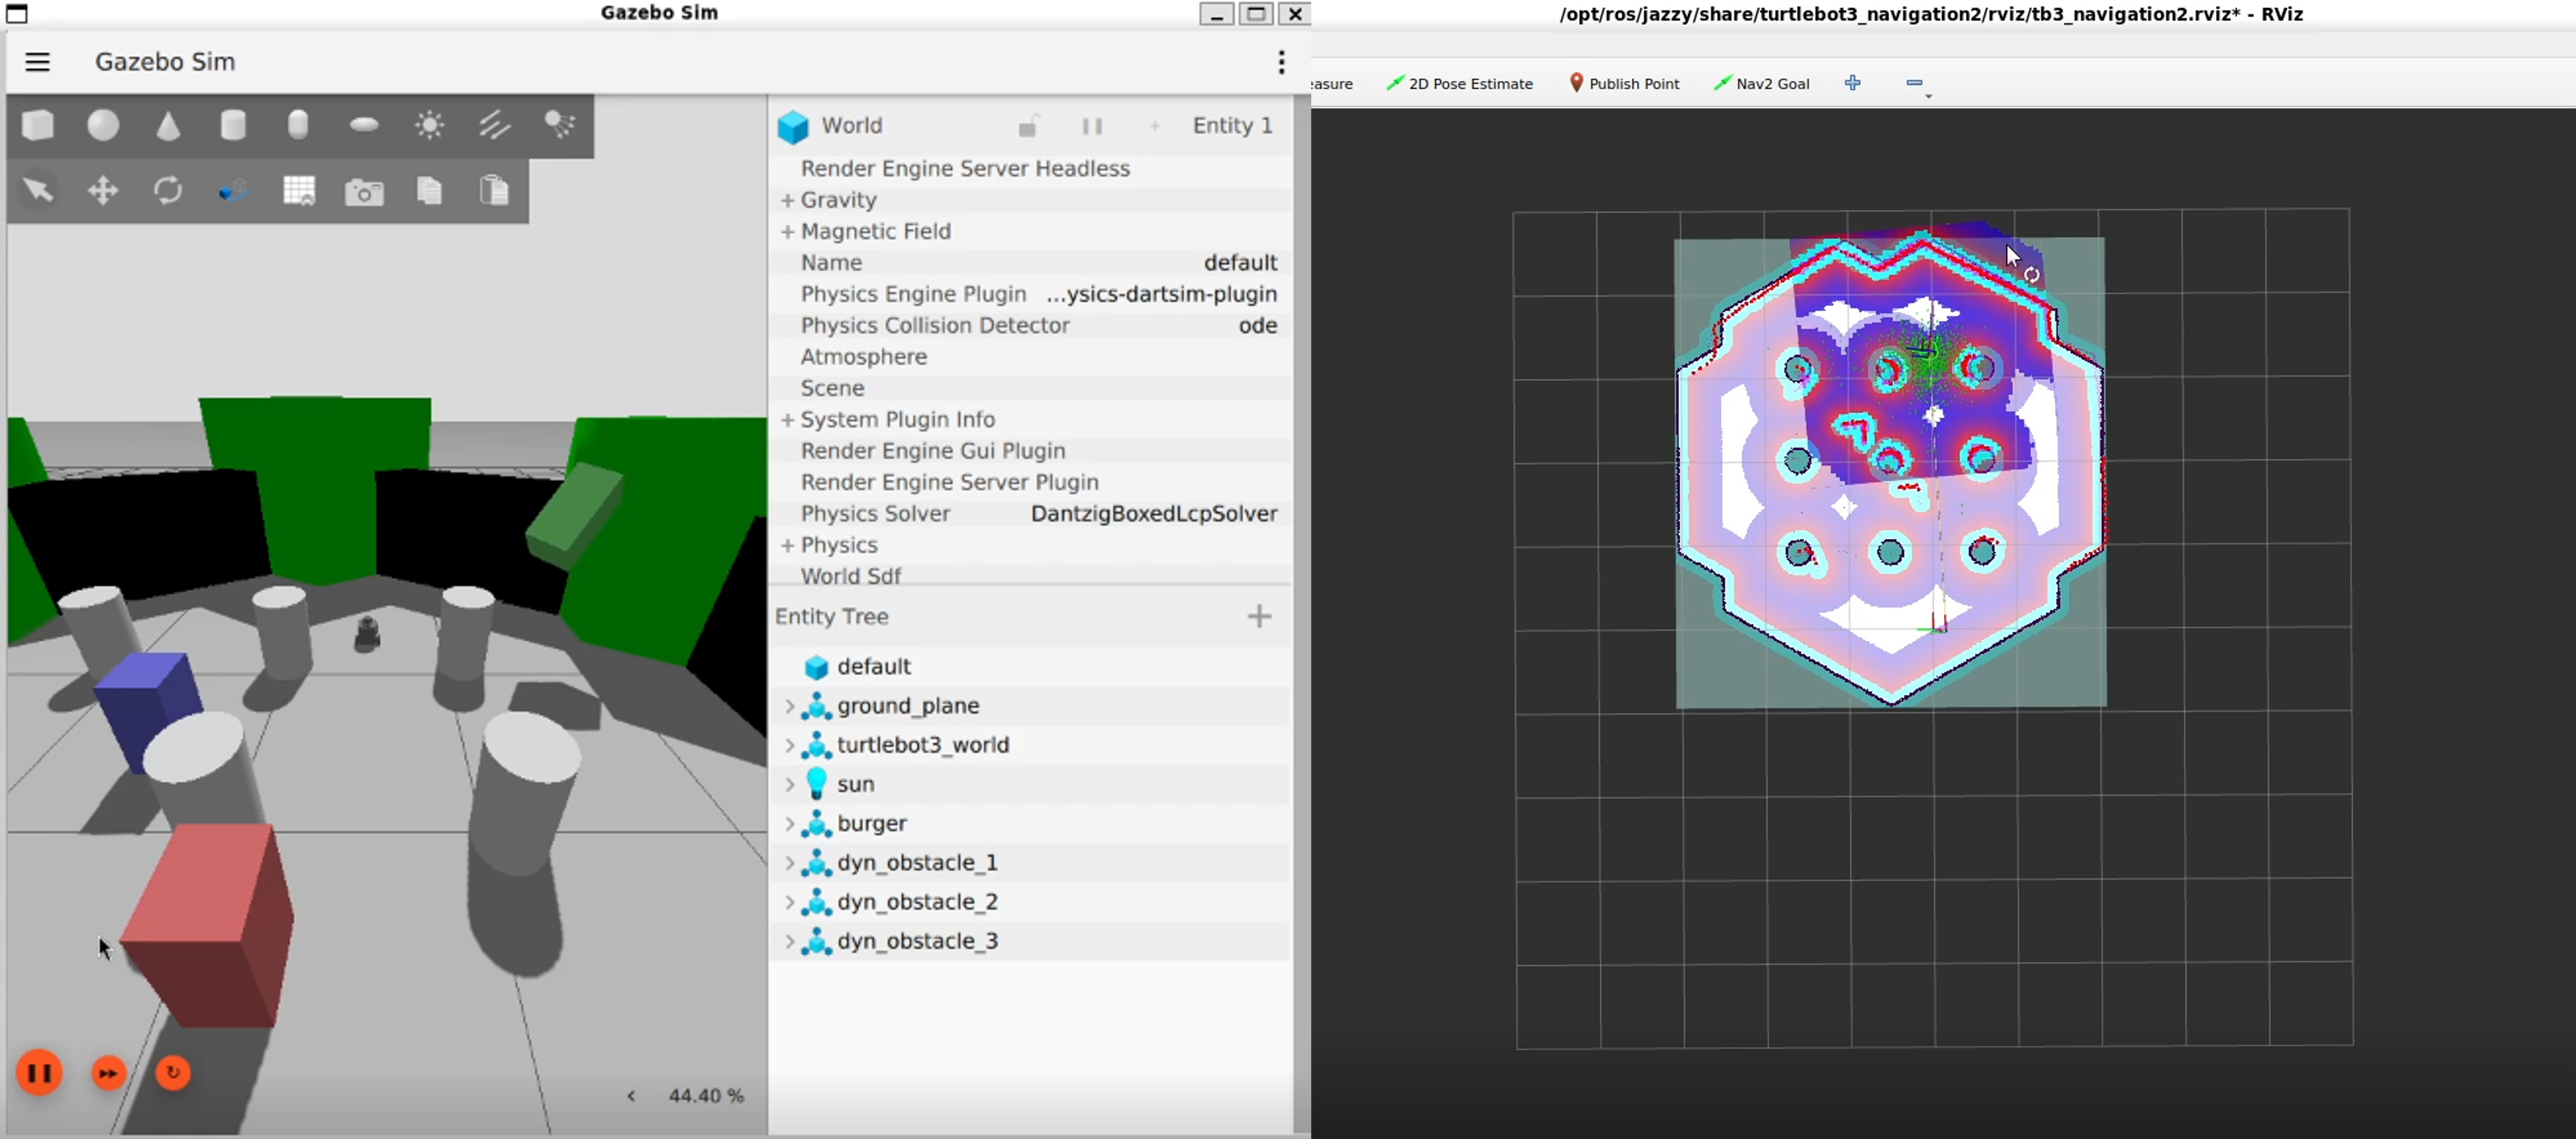
\includegraphics[width=\linewidth]{moving_obj.png}
        \footnotesize{Moving obstacles during navigation.}
    \end{columns}
\end{frame}

% =============================================================
% Section: Conclusion
% =============================================================
\section{Conclusion}
\begin{frame}{11. Conclusion}
    \begin{itemize}
        \item Completed a full simulation pipeline: Gazebo + RViz2 + SLAM mapping.
        \item Integrated Nav2 on the saved map for autonomous goal navigation.
        \item Added extensions: OS contention analysis and dynamic moving obstacles for more realistic testing.
    \end{itemize}

    \vspace{0.4cm}
    \centering
    \begin{block}{Next Steps}
        Expand to more complex worlds, tune Nav2 costmaps, and evaluate policies under heavier dynamic scenes.
    \end{block}
\end{frame}

\begin{frame}
    \centering
    \Huge Thanks for listening!
\end{frame}

\end{document}
